%% =========================================================================
\section{Results}\label{sec:results}

\draftnote{Writing guide (2026-07-11, verified against a fresh
\texttt{ablation.py} run; updated 2026-07-12 after the \texttt{rates.py}
run): each subsection below carries a \texttt{\%\%} comment block with the
concrete numbers to write from and the narrative beats, in the order we
agreed. Sections~\ref{sec:overlap}--\ref{sec:kmd} are fully backed by
\texttt{results/} and ready to draft now; \ref{sec:missingness} is
optional-now (data-quality preamble); \ref{sec:rate-vs-stock}
and~\ref{sec:build-comparison} are now backed by
\texttt{results/rates\_*.csv} (2026-07-12) and drafted below. Draft order:
overlap $\to$ annual $\to$ discontinued $\to$ area $\to$ KMD $\to$ rates.}

%% ---- SOURCE FILES (real names, verified) --------------------------------
%%   results/ablation_summary.csv  — one row / 12 variants: counts + 3 area
%%                                   defs (footprint/total/etage) w/ median
%%                                   + coverage%%
%%   results/annual.csv            — variant x year: count + m2 per area def
%%   results/by_region.csv         — variant x region: count + etage m2
%%   results/overlap.csv           — pairwise intersection + Jaccard (D1-D6)
%%   results/overlap_2018_2025.csv — same, restricted to dated 2018-2025
%%   results/kmd_comparison.csv    — each proxy vs KMD extract (raw + window)
%%   results/cleaning_report.csv   — cleaned values per rule, per indicator
%%   results/data_quality_*.csv    — from src/data_quality.py (NOT ablation)
%%   results/rates_summary.csv     — variant x window: mean rate + coverage
%%                                   + m2/yr, both pairings (src/rates.py)
%%   results/rates_spread.csv      — window x pairing: min/max variant + fold
%%   results/rates_annual.csv      — variant x year 2011-2025: rate series
%%   results/stock_national.csv    — parsed BYGB34 national stock per year
%%   results/figures/*.png|pdf     — annual_counts, annual_area_total,
%%                                   overlap_heatmap, overlap_heatmap_2018_2025
%%                                   (rate_vs_stock came from src/rates.py, which is
%%                                   not in this checkout — regenerate before reuse)

\subsection{Indicator overlap}\label{sec:overlap}
%% STATUS: READY. Sources: overlap.csv + counts from ablation_summary.csv.
%%   Figure: results/figures/overlap_heatmap.png. This is the SPINE of the
%%   paper — the proxies genuinely disagree; everything downstream is the
%%   consequence. Lead with it.
%% NARRATIVE BEATS:
%%  1. COUNT SPREAD. The six indicators, same window (2000-2025), same
%%     extract, disagree by a factor of ~4.4x on how many buildings were
%%     demolished:
%%        D1 status=10                 436,194   (most inclusive)
%%        D4 sagstype=32               237,012
%%        D6 total case, sag002 dated  231,962
%%        D2 forretningsproces=3       225,706
%%        D5 status10 & sagstype=32    200,634
%%        D3 status10 & proces=3        99,664   (least inclusive)
%%     Even the two "canonical" single signals — register-exit (D1) vs
%%     event-code (D2) — differ nearly 2x.
%%  2. THE TWO CANONICAL PROXIES BARELY AGREE. D1 vs D2 Jaccard = 0.177;
%%     their intersection is only 99,664 buildings (= all of D3). So
%%     status=10 and forretningsproces=3 identify largely DIFFERENT
%%     buildings. D2 is NOT a subset of D1: 126k buildings are process-3
%%     but never status-10 (report from docs; = 225,706 - 99,664).
%%  3. THE CASE-BASED FAMILY IS TIGHT. D4/D5/D6 cluster at Jaccard
%%     0.85-0.92: D4-D6 0.918, D5-D6 0.853, D4-D5 0.847. So "which
%%     demolition-case variant" barely matters; "case-based vs
%%     register-exit vs event-code" matters enormously.
%%  4. CROSS-FAMILY LOW: D1 vs case-family ~0.42-0.46 (D1-D5 0.460,
%%     D1-D4 0.425, D1-D6 0.424); D2 vs everything 0.18-0.44.
%%  INTERPRETATION: the choice of proxy is not cosmetic. Disagreement
%%  between indicators IS the result, not noise to resolve against a
%%  reference (there is no gold label — see indicators section).
The six indicators pick out very different sets of demolished buildings
(Table~\ref{tab:overlap-size}). The count ranges from 99{,}664 buildings
(D3) to 436{,}194 (D1) --- a 4.4-fold difference --- and their total floor
area (\texttt{byg038}) ranges from 13.5 to 44.7~million~m\textsuperscript{2}.
The area figures depend not only on which buildings an indicator selects,
but also on how many of them have a recorded area, and that share differs
by indicator (Section~\ref{sec:area-sensitivity}).

\begin{table}[htbp]
\centering
\caption{Number of demolished buildings and their total floor area
(\texttt{byg038}) under each indicator, 2000--2025.}
\label{tab:overlap-size}
\begin{tabular}{llrr}
\toprule
Indicator & Signal & Buildings & Floor area (M\,m\textsuperscript{2}) \\
\midrule
D1 & \texttt{status = 10}                    & 436{,}194 & 44.7 \\
D2 & \texttt{forretningsproces = 3}          & 225{,}706 & 16.1 \\
D3 & D1 $\cap$ D2                            &  99{,}664 & 13.5 \\
D4 & \texttt{sagstype = 32}                  & 237{,}012 & 34.5 \\
D5 & D1 $\cap$ D4                            & 200{,}634 & 26.6 \\
D6 & \texttt{sagstype = 32}, notification date & 231{,}962 & 33.7 \\
\bottomrule
\end{tabular}
\end{table}

Figure~\ref{fig:overlap-heatmap} shows how much the sets overlap, measured
by the Jaccard index (the buildings two indicators share, divided by the
number in either one). D1 (\texttt{status = 10}) and D2
(\texttt{forretningsproces = 3}) overlap by only 0.18: they share 99{,}664
buildings, which means 126{,}042 of D2's buildings never reach
\texttt{status = 10}. The three demolition-case indicators D4, D5 and D6
overlap each other much more, at 0.85--0.92, while each overlaps D1 at
0.42--0.46 and D2 at 0.28--0.30.

\begin{figure}[htbp]
\centering
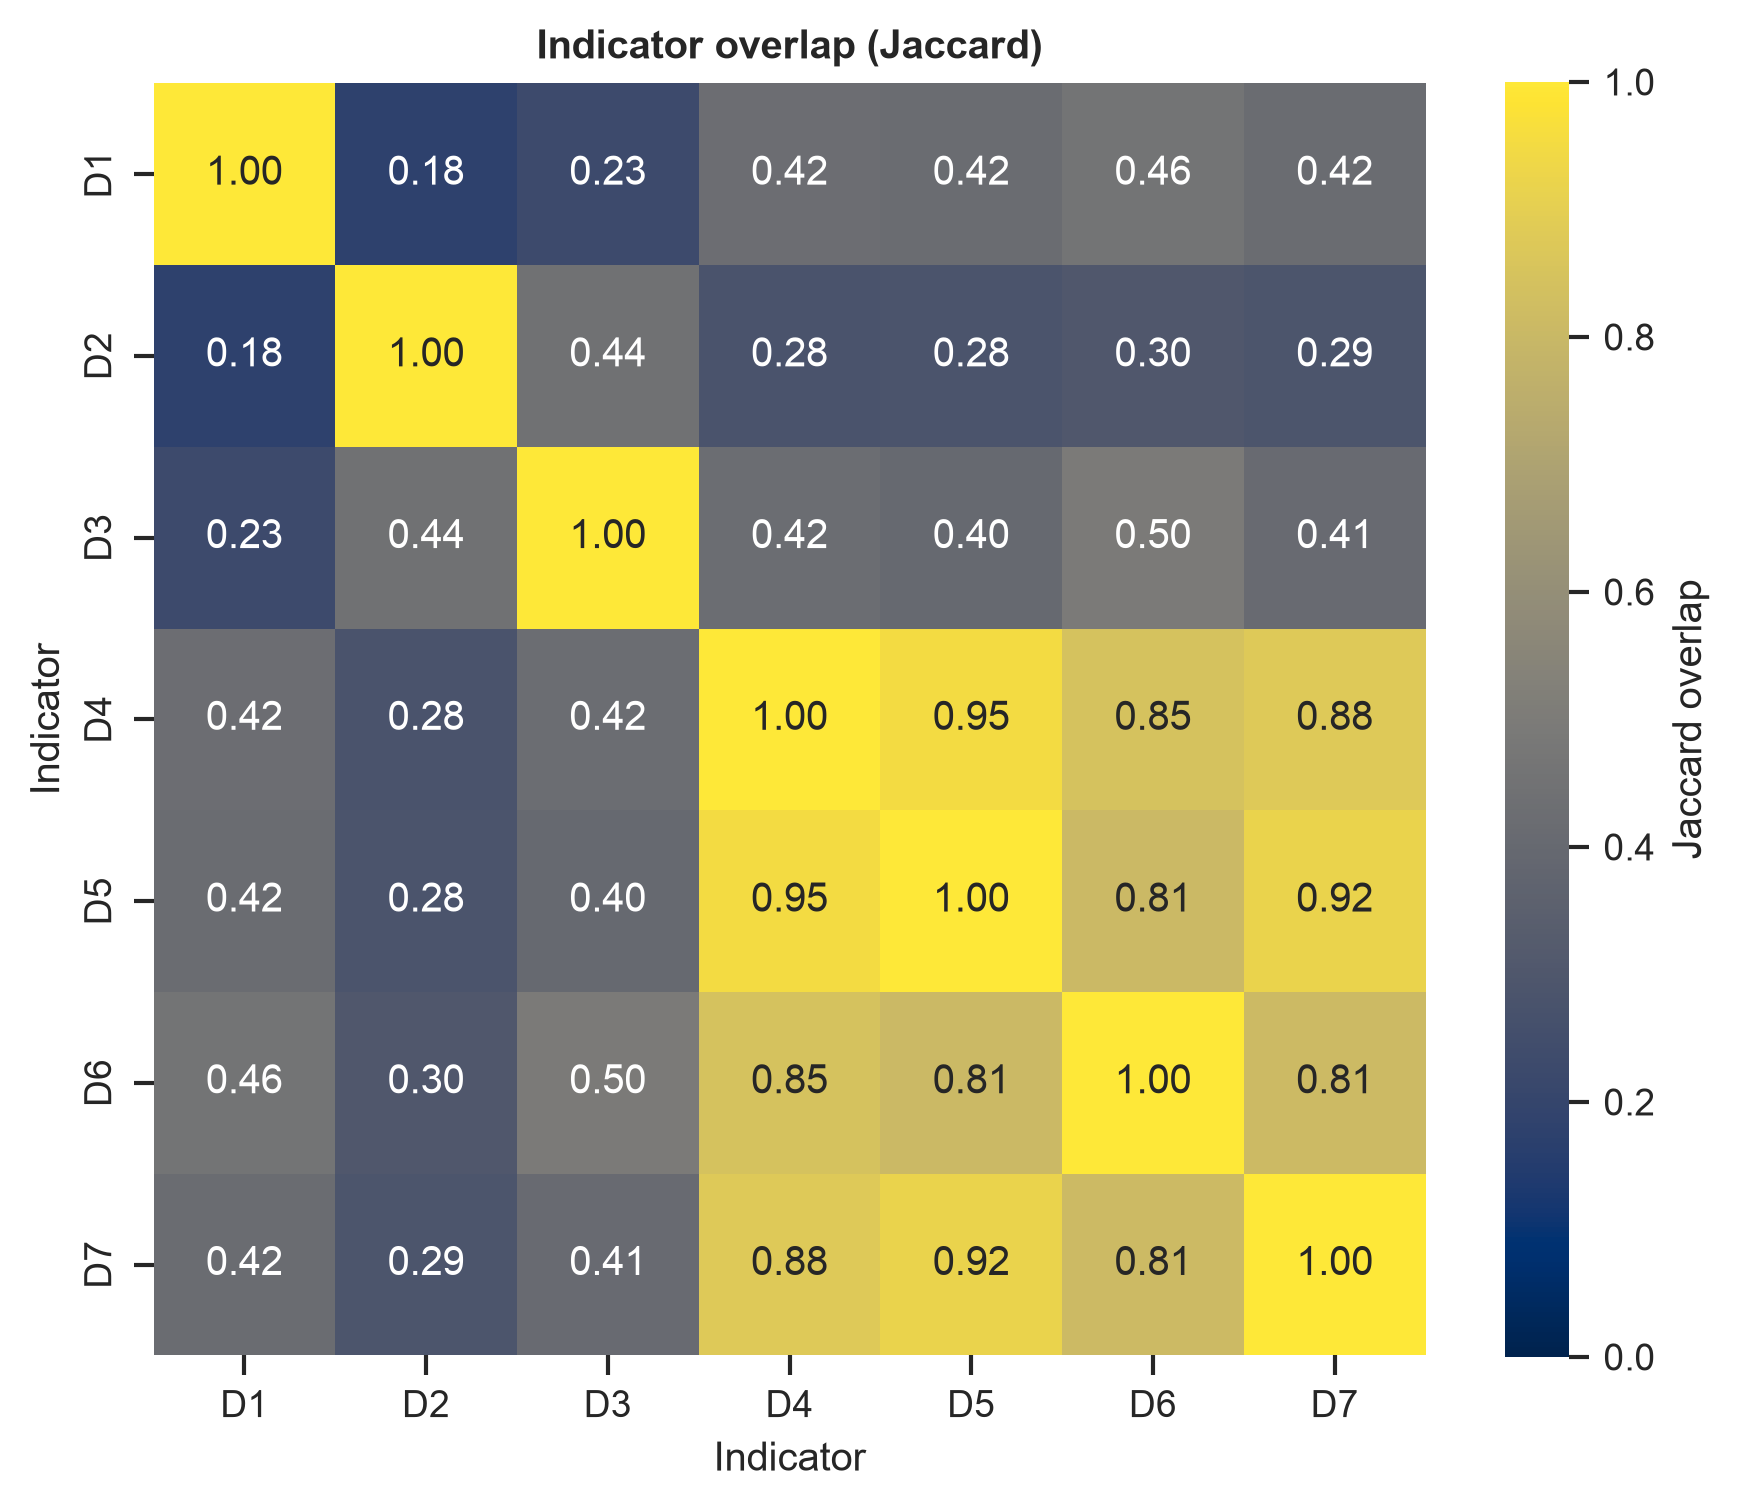
\includegraphics[width=0.7\textwidth]{media/overlap_heatmap.png}
\caption{How much the six indicators' sets of demolished buildings
overlap, measured by the Jaccard index (2000--2025).}
\label{fig:overlap-heatmap}
\end{figure}

Restricting the comparison to dated memberships in the stable 2018--2025
window changes the pattern but not the main conclusion
(Figure~\ref{fig:overlap-heatmap-2018}). The inclusive register-exit
indicator D1 remains the broad outlier: its overlap with D2 is 0.38 and
with the total-demolition-case indicators D4/D5 is 0.42. By contrast,
D2, D3, D4 and D5 form a much tighter recent-period cluster, with
Jaccard values of 0.87--1.00. This shows that part of the weak full-window
agreement is a period and dating issue rather than only a membership
issue. In this dated-window table D4 and D5 are identical because D4 is
dated by the building's status-10 year; D4 case-only members without a
status-10 year are therefore excluded from the windowed comparison. The
notification-dated case indicator D6 overlaps the same cluster
less strongly, at 0.65--0.67, because it assigns the year from the case
date rather than from the status-10 register exit.

\begin{figure}[htbp]
\centering
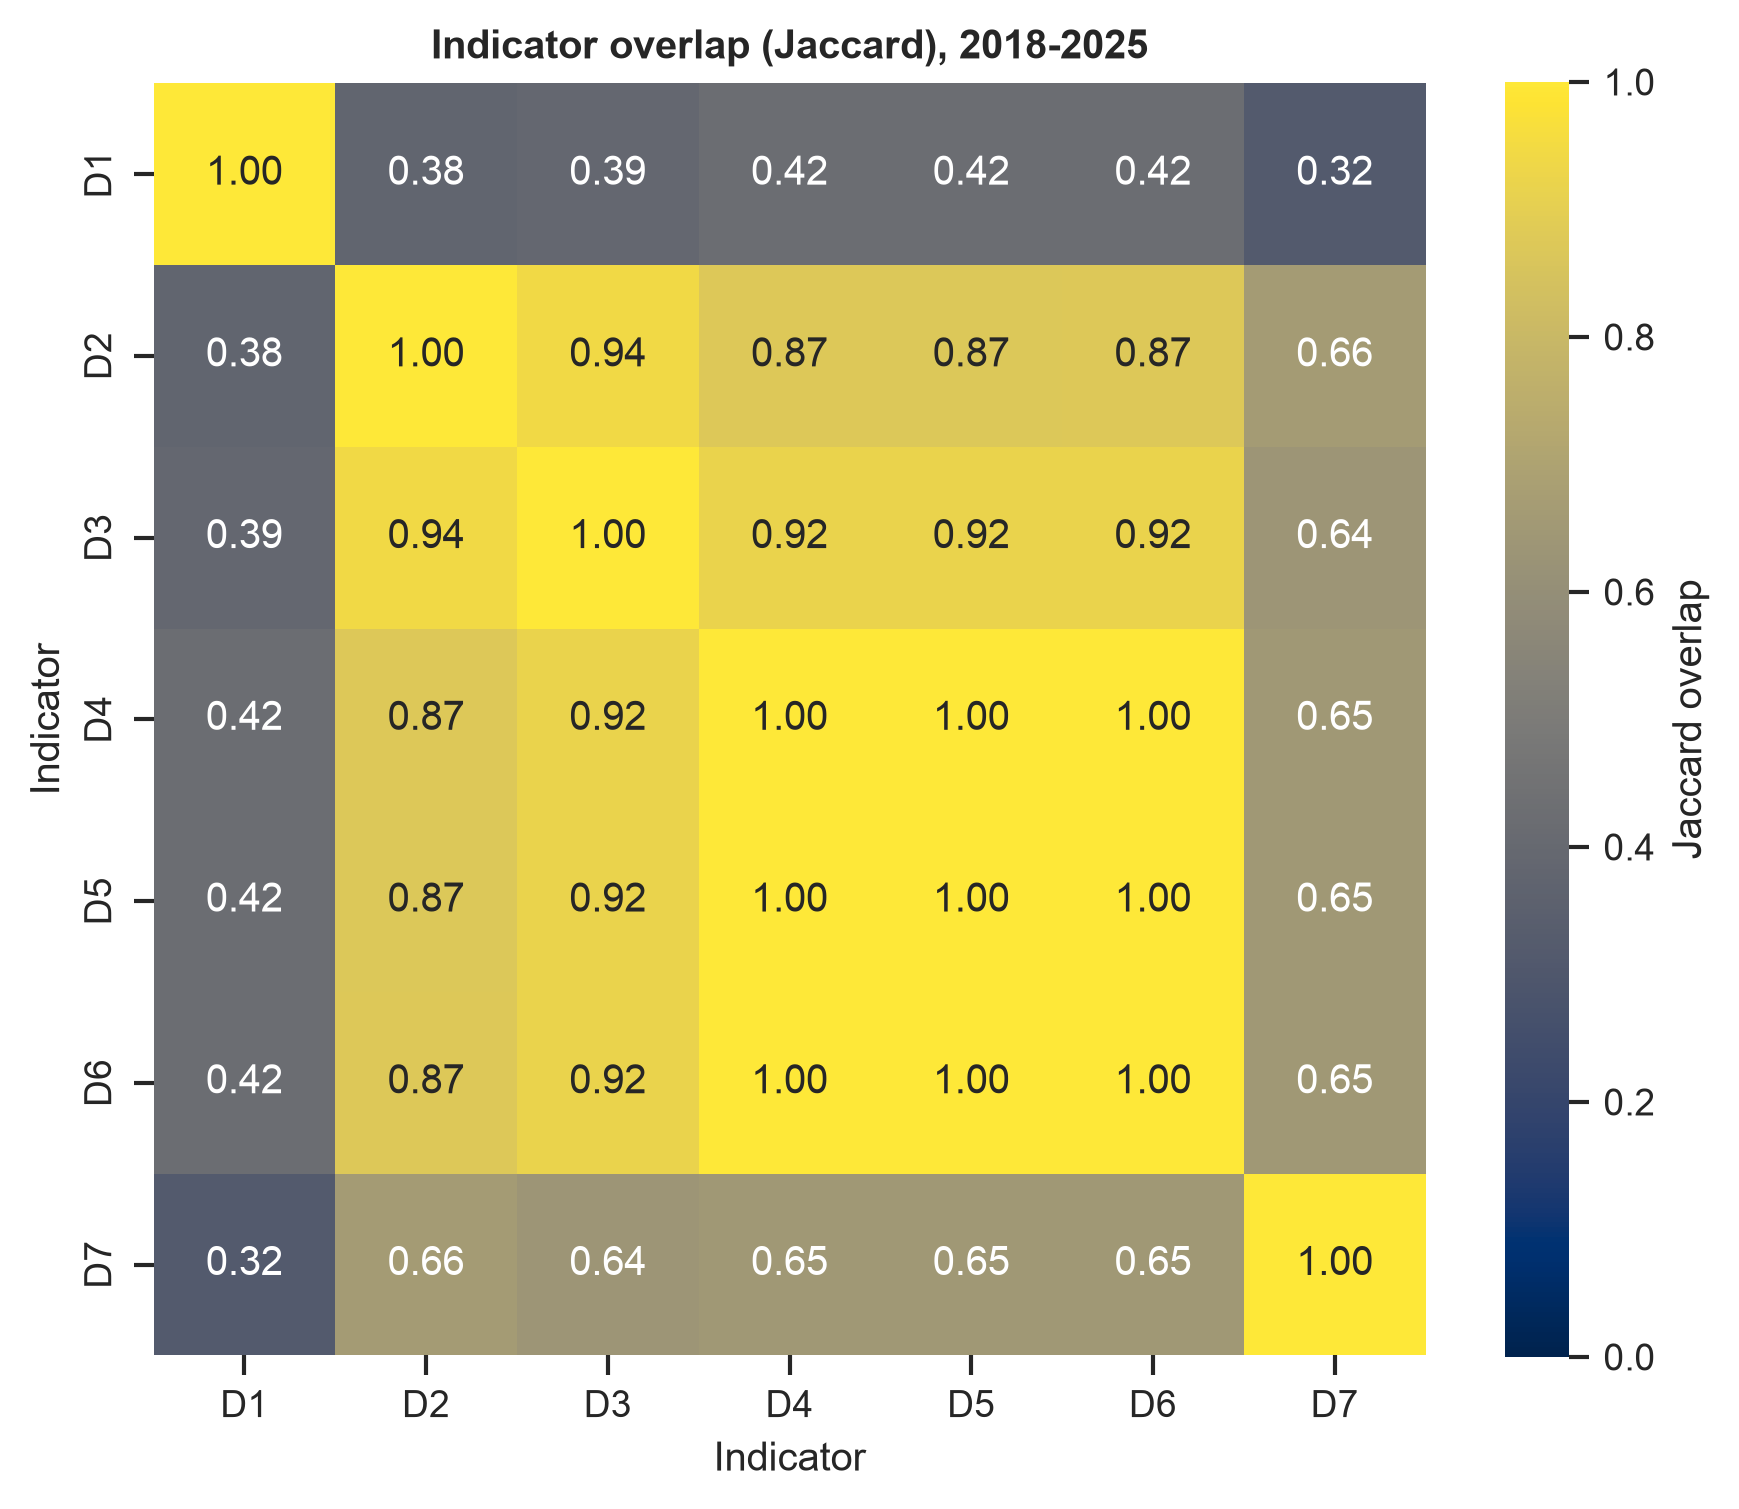
\includegraphics[width=0.7\textwidth]{media/overlap_heatmap_2018_2025.png}
\caption{Indicator overlap restricted to dated memberships in the
2018--2025 comparison window. The higher agreement among D2--D5 shows the
recent-period convergence of the process and case-based signals; D6 is
partly separated by its notification-date clock.}
\label{fig:overlap-heatmap-2018}
\end{figure}

\subsection{Annual demolition estimates by indicator}\label{sec:rates}
%% STATUS: READY. Sources: annual.csv (+ ablation_summary totals).
%%   Figures: annual_counts.png, annual_area_total.png. This is the
%%   ablation's payload: same computation, swap indicator, watch the
%%   national series move.
%% NARRATIVE BEATS:
%%  1. THE SPREAD PERSISTS EVERY YEAR. For a representative recent complete
%%     year (2022): D1=32,874 buildings, D4=16,026, D6=13,033.
%%     Report the annual count envelope across indicators, not one line.
%%  2. AREA/YR ENVELOPE (byg038 total m2): 2018-2025 means run 2.84M m2/yr
%%     for D1, 1.72M for D4/D5, 2.14M for D6. Give the range; this is
%%     what feeds any stock-turnover / LCA reference figure.
%%  3. TWO ARTIFACTS TO CAVEAT (do NOT hide these):
%%     (a) YEAR-2000 PILE-UP. Backdated virkningFra below the 2000 clamp
%%         all lands on 2000: D1=24,550 in 2000 vs ~300-1,600/yr for
%%         2001-2010; D4=14,056 in 2000. D6 (notification-dated) does NOT
%%         pile up (25 in 2000) — good illustration that the artifact is a
%%         register-exit dating effect, not real activity. => the
%%         comparable window is ~2011/2012-2025, not 2000.
%%     (b) 2011 STEP-UP. All register-exit series jump at 2011 (BBR
%%         registration reforms) — pre-2011 is not comparable.
%%  4. UNDATED CASE MEMBERS. D4 has members with no status-10 year, so
%%     they sit in the totals but not the time series: D4 n_dated=200,634
%%     of 237,012 (D4's dated subset = D5). State this so the annual D4
%%     line reads lower than its total.
%%  WINDOW DECISION: Section~\ref{sec:data} defines 2000--2025 as the full
%%  reporting window and 2018--2025 as the main comparison window.
Figure~\ref{fig:annual} shows the demolitions per year under each
indicator: counts in panel~(a) and demolished total floor area in
panel~(b), across the full 2000--2025 window. The differences between
indicators seen in Section~\ref{sec:overlap} continue year by year: the
curves have the same shape but stay separated by roughly the same multiple
throughout. We compare numbers only over the complete years 2018--2025
(Section~\ref{sec:methods}), where all indicators are reliable;
Table~\ref{tab:annual-mean} gives each indicator's average over those eight
years.

\begin{table}[htbp]
\centering
\caption{Average demolitions per year and demolished floor area per year
(\texttt{byg038}) under each indicator, 2018--2025.}
\label{tab:annual-mean}
\begin{tabular}{llrr}
\toprule
Indicator & Signal & Buildings/yr & Floor area (M\,m\textsuperscript{2}/yr) \\
\midrule
D1 & \texttt{status = 10}              & 30{,}369 & 2.84 \\
D2 & \texttt{forretningsproces = 3}    & 12{,}458 & 1.89 \\
D3 & D1 $\cap$ D2                      & 11{,}748 & 1.60 \\
D4 & \texttt{sagstype = 32}            & 12{,}708 & 1.72 \\
D5 & D1 $\cap$ D4                      & 12{,}708 & 1.72 \\
D6 & \texttt{sagstype = 32}, notification date & 14{,}433 & 2.14 \\
\bottomrule
\end{tabular}
\end{table}

Over 2018--2025 the yearly count runs from about 11{,}700 (D3) to
30{,}400 (D1). In every single year the highest indicator is 2.2 to 3.1
times the lowest. D1 sits at roughly twice the demolition-case indicators,
which group near 12{,}700/yr (D4 and D5); D6 is a little higher, at
about 14{,}400/yr. The gap in demolished area is smaller: yearly totals
average 1.6 to 2.8~million~m\textsuperscript{2}. D1's area is only about
1.6 times the case indicators, less than its 2.4-times lead in counts --- so
the extra buildings D1 picks up tend to be smaller and less often have a
recorded area (Sections~\ref{sec:overlap} and~\ref{sec:area-sensitivity}).

The years before 2011 are not comparable and are shown only for
completeness, because of two dating effects. First, dates that were
backdated to before the start of the window all pile up on the year 2000:
D1 shows 24{,}550 buildings in 2000 against 600--1{,}150 per year in the
mid-2000s, and D4 shows 14{,}056. D6, which is dated from the demolition
notice, shows no such spike (25 in 2000). Second, the register-exit and
case indicators jump upward in 2011, after a BBR registration reform (D1:
1{,}150 in 2010, 12{,}670 in 2011, 22{,}546 in 2012). D6 instead already
has large counts in 2009--2010, when the others are close to zero --- these
are the same demolitions, but dated from the notice rather than from the
register exit. So the indicators disagree not only on which buildings count
as demolished, but also on \emph{when} the demolition happened.

Finally, the demolition-case indicator D4 includes buildings that
never reached \texttt{status = 10} and so have no year attached: 200{,}634
of D4's 237{,}012 buildings have a date. The undated ones count toward the
totals in Table~\ref{tab:overlap-size} but not toward the yearly series, so
D4's yearly line sits below its total and matches D5.

\begin{figure}[htbp]
\centering
\begin{subfigure}[t]{0.49\textwidth}
  \centering
  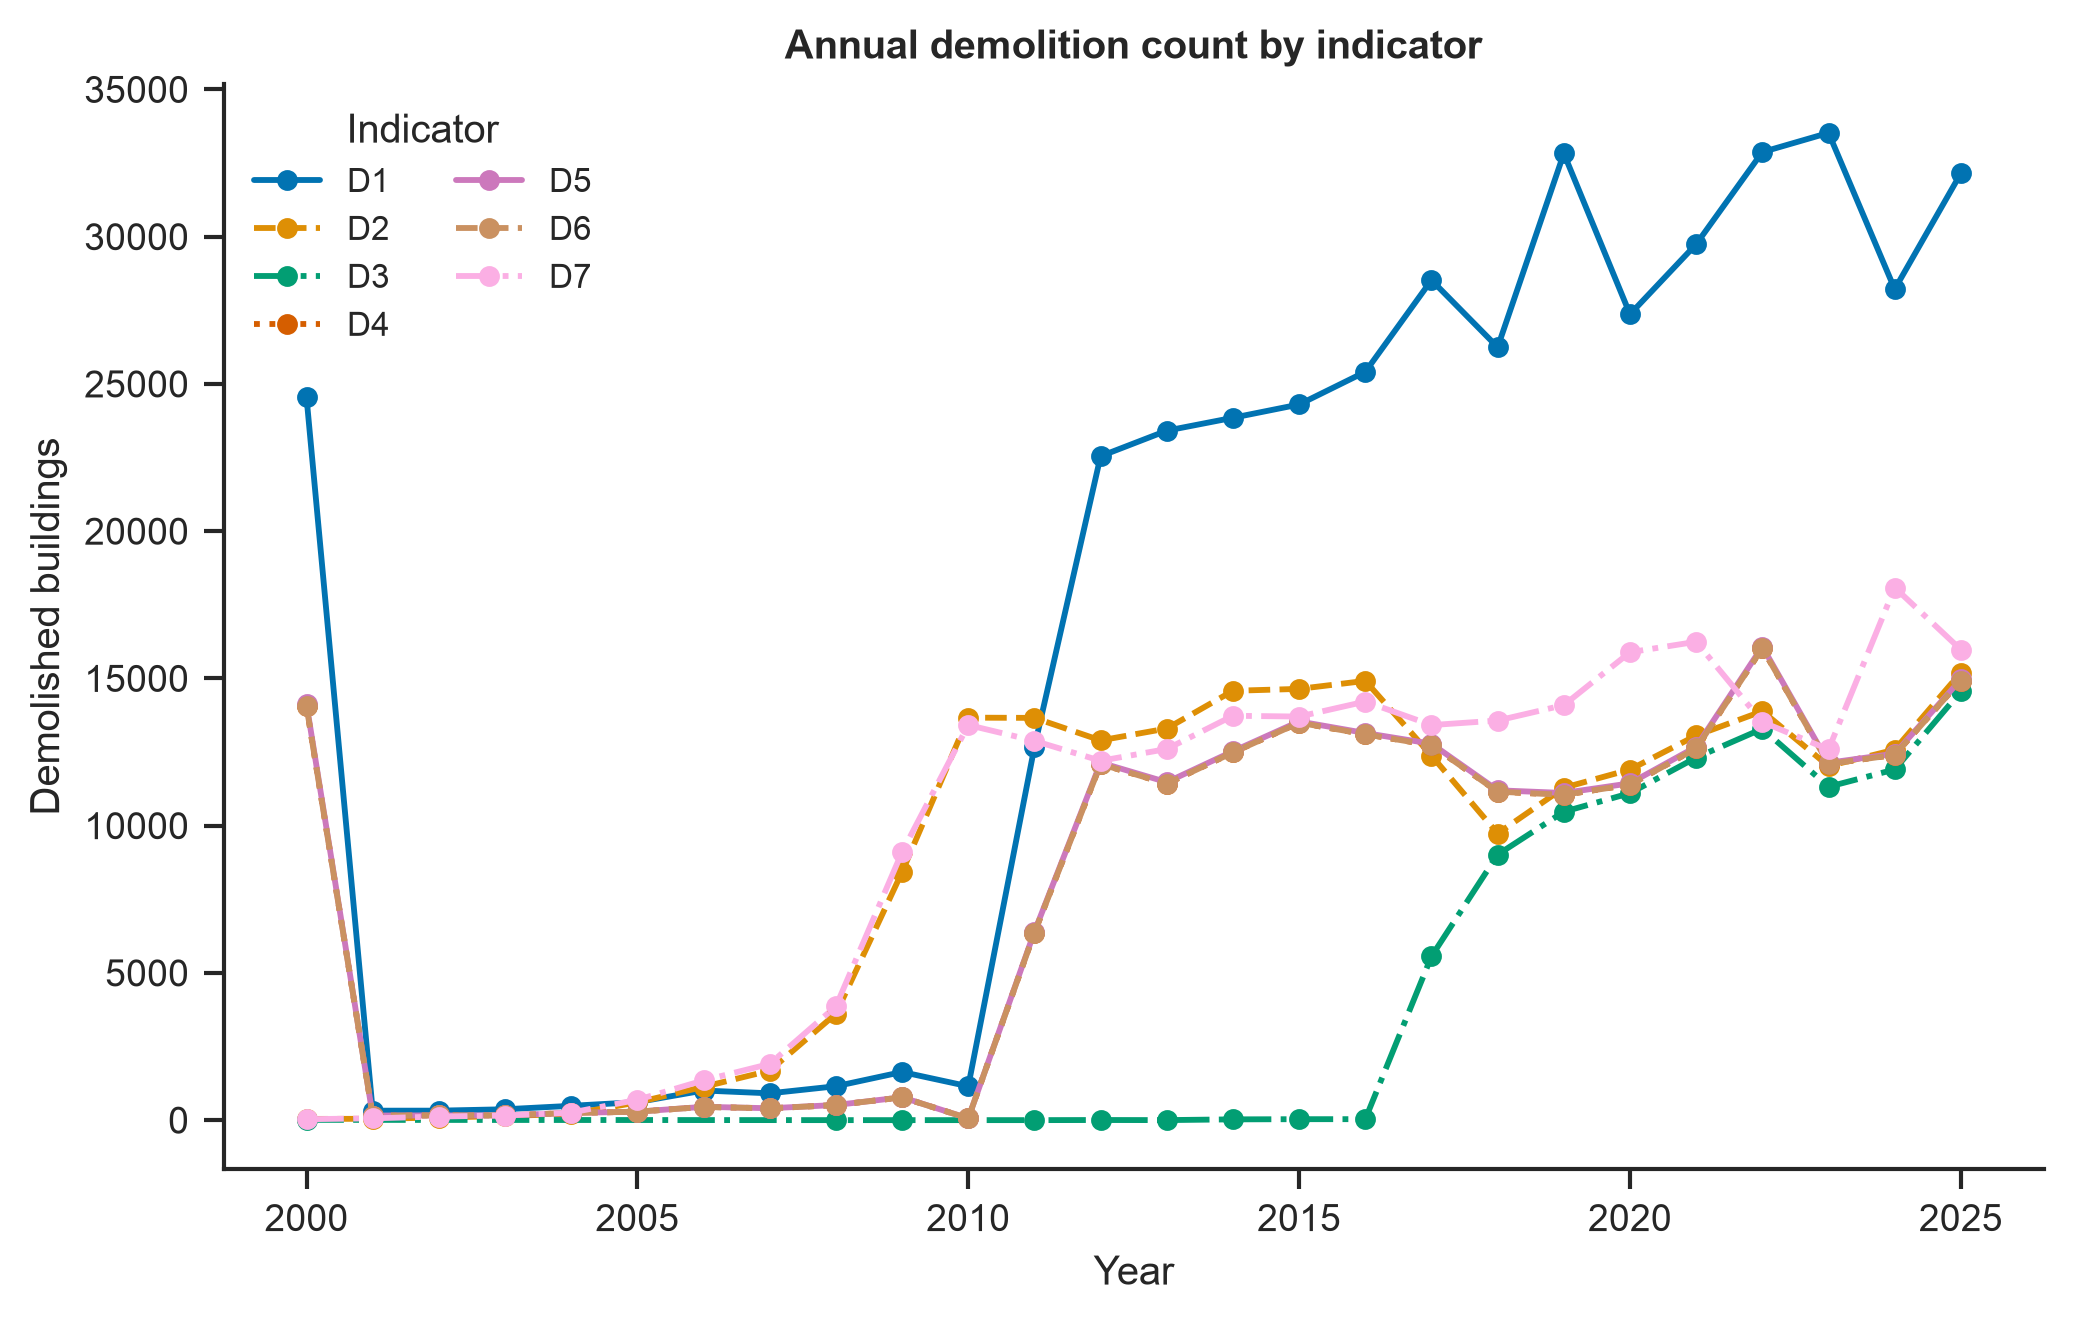
\includegraphics[width=\textwidth]{media/annual_counts.png}
  \caption{Demolition counts.}
  \label{fig:annual-counts}
\end{subfigure}
\hfill
\begin{subfigure}[t]{0.49\textwidth}
  \centering
  
\includegraphics[width=\textwidth]{media/annual_area_total.png}
  \caption{Demolished floor area.}
  \label{fig:annual-area}
\end{subfigure}
\caption{Annual demolition series per indicator, 2000--2025:
(a)~building counts and (b)~demolished floor area.}
\label{fig:annual}
\end{figure}

\subsection{Discontinued-code analysis}\label{sec:discontinued}
%% STATUS: READY. Sources: the -exdisc variants in ablation_summary.csv.
%%   THE STRONGEST SELF-CONTAINED FINDING. Headline: the discontinued-code
%%   exclusion is an AREA story, not a count story.
%% NARRATIVE BEATS:
%%  1. COUNTS MOVE MODESTLY, AREA COLLAPSES. Excluding discontinued round-
%%     number use-codes from D1:
%%        count   436,194 -> 302,261   (-31%)
%%        etage   47.5M  -> 9.9M m2     (-79%)
%%        total   44.7M  -> 9.1M m2     (-80%)
%%        footprint 50.1M -> 15.5M m2   (-69%)
%%     A one-third count cut wipes out four-fifths of the demolished area.
%%  2. UNIFORM STRIP = BASE RATE, NOT ARTIFACT. The exclusion removes
%%     ~31-35% of EVERY indicator's buildings (D4 237,012->155,299 = -34%).
%%     That uniformity says ~a third of the stock carries these old
%%     agricultural/industrial codes — a base rate, not concentrated
%%     re-registration artifacts (contrast the thesis's >90%-fake premise).
%%  3. WHAT IT REMOVES IS THE BIG BUILDINGS. The excluded round-number
%%     codes are large agricultural structures carrying disproportionate
%%     m2 — matches BUILD's finding that landbrug dominates demolished
%%     area. (Median etage m2 also drops, D1 117 -> 100.)
%%  4. IT ALSO REMOVES GENUINE DEMOLITIONS. Of the status-10 buildings the
%%     exclusion drops, 50.7% ALSO carry a formal demolition case (vs 44.2%
%%     among those it keeps) — so it over-corrects. (methods sec covers
%%     this; keep the empirical claim here.)
%%  INTERPRETATION: any headline demolished-m2 figure is hostage to this
%%  single filter choice — a decision that barely moves the building count.
%%  Whether the exclusion is a "correction" is unresolved (settle vs
%%  BOSSINF, future work), so we report inclusive AND excluded side by side.
\pending{inclusive vs -exdisc counts and area for each indicator; the
count-vs-area asymmetry (-31\% count / -79\% area on D1)}

\subsection{Total-floor-area coverage and robustness}\label{sec:area-sensitivity}
%% STATUS: READY for the old 3-area run, but needs final rewrite once the
%%   main pipeline is aligned with the A2 decision. Main text should focus on
%%   byg038 coverage by indicator; footprint and etage are robustness /
%%   appendix material, not co-equal headline outcomes.
%% NARRATIVE BEATS:
%%  1. MAIN POINT: byg038 is the primary area outcome, but coverage is limited
%%     and must be reported next to every demolished-m2 estimate.
%%  2. COVERAGE DEPENDS ON THE INDICATOR. Floor-area coverage is
%%     ~44-47% on D1 (status-10) but ~61-62% on the case-based indicators
%%     (D4 total coverage 62.0%, D6 62.3%) — the register-exit proxy sweeps
%%     in more attribute-poor stub records.
%%  3. ROBUSTNESS / APPENDIX: footprint is nearly complete but is a different
%%     physical measure; byg039+byg040 is useful for BUILD comparison but is a
%%     constructed area definition. These alternatives can be shown briefly in
%%     appendix/supplement to demonstrate that they do not replace byg038.
\pending{rewrite around byg038 coverage by indicator; move footprint and
byg039+byg040 comparison to appendix/supplement or a short robustness note}

\subsection{External anchor: the KMD/Andersen extract}\label{sec:kmd}
%% STATUS: READY. NEW subsection (was not in the plan scaffold). Source:
%%   kmd_comparison.csv. This is external validation, not ground truth —
%%   frame it as "which proxy is the field's reference actually equal to?"
%% SETUP: the KMD/Andersen extract (152,300 rows, 2000-2020) is the
%%   nearest-to-truth national reference the literature leans on. We hold
%%   the raw file; every row is Sagstype=32 (total demolition). We score
%%   each proxy against it, window-matched to 2011-2019 (both sides dated by
%%   status-10 virkningFra) — the fair comparison; raw is in the CSV too.
%% RESULTS (window_2011_2019 rows):
%%     proxy   recall  precision  Jaccard
%%     D1      1.000   0.472      0.472   <- strict SUPERSET (~2x overcount)
%%     D2/D3   0.242   0.997      0.242   <- severe UNDERCOUNT (~4x)
%%     D4      0.997   0.994      0.991   <- ~ KMD
%%     D5      0.997   0.994      0.991   <- ~ KMD (identical to D4 in-window)
%%     D6      0.990   0.995      0.985
%% THREE-TIER CONCLUSION (keep distinct, do not overclaim):
%%  - PINNED: KMD is the total-demolition-CASE signal, and it is NOT
%%    status=10. D1 contains KMD (100% recall) but flags ~2x as many
%%    (47% precision) => superset. D2 ruled out the other way (24% recall).
%%  - UNDERDETERMINED: D4 ~= D5 ~= D6 all reproduce KMD to 0.985-0.991;
%%    membership cannot single one out (D4/D5 identical in-window, the
%%    status-10 clock forces it). Claim "KMD = the total-demolition case
%%    family," D4/D5 tightest — NOT "KMD = D4".
%%  - STILL UNKNOWN: KMD's pre-2011 filtering / dedup recipe (unpublished).
%%  WHY IT MATTERS: independently confirms the two tradeoff claims —
%%  status=10 overcounts ~2x, process=3 undercounts ~4x — against a signal
%%  we can build and document ourselves. Belongs as a window-matched anchor,
%%  not a gold label.
The literature's nearest-to-truth national reference is the KMD/Andersen
demolition extract~\cite{andersen2022adaptation}: 152{,}300 demolition
cases spanning 2000--2020, compiled by the former BBR administrator (KMD)
under a filtering recipe that was never published. We hold the raw file,
and every row in it carries \texttt{sagstype = 32} (total demolition). This
lets us turn an opaque reference into a measurement: rather than treat the
extract as ground truth, we ask which of our transparent indicators it
actually coincides with. We score each indicator against the extract by
recall (the share of KMD buildings it recovers), precision (the share of
its own buildings that are in KMD) and the Jaccard index, window-matched to
2011--2019 --- the years both sides date on the same \texttt{status = 10}
clock (Table~\ref{tab:kmd}).

\begin{table}[htbp]
\centering
\caption{Each indicator scored against the KMD/Andersen demolition extract
(every case \texttt{sagstype = 32}), window-matched to 2011--2019.}
\label{tab:kmd}
\begin{tabular}{llrrr}
\toprule
Indicator & Signal & Recall & Precision & Jaccard \\
\midrule
D1 & \texttt{status = 10}              & 1.000 & 0.472 & 0.472 \\
D2 & \texttt{forretningsproces = 3}    & 0.242 & 0.997 & 0.242 \\
D3 & D1 $\cap$ D2                      & 0.242 & 0.997 & 0.242 \\
D4 & \texttt{sagstype = 32}            & 0.997 & 0.994 & 0.991 \\
D5 & D1 $\cap$ D4                      & 0.997 & 0.994 & 0.991 \\
D6 & \texttt{sagstype = 32}, notification date & 0.990 & 0.995 & 0.985 \\
\bottomrule
\end{tabular}
\end{table}

The comparison splits the indicators into three groups. First, the two
canonical single signals bracket the extract from opposite sides.
\texttt{status = 10} (D1) recovers every KMD building (recall 1.000) but
flags roughly twice as many (precision 0.472): a strict superset that
overcounts about twofold. \texttt{forretningsproces = 3} (D2, and D3 with
it) does the reverse, catching only a quarter of KMD (recall 0.242) at
near-perfect precision --- an undercount of about fourfold. The extract is
therefore neither of the two proxies the literature has leaned on as
canonical: it is a demolition-\emph{case} signal, not a register-exit one.

Second, the three case-based indicators all reproduce the extract almost
exactly: D4, D5 and D6 reach Jaccard 0.985--0.991, with recall and
precision both above 0.99. Membership alone cannot single one of them out:
D4 and D5 are identical within the window, because both sides are dated on
the same \texttt{status = 10} clock there, and D6 --- dated by the case
notification instead --- matches almost as closely. The finding is thus
that the extract corresponds to the case \emph{family} D4--D6, not to any
single indicator.

Third, what stays unknown is the extract's own construction: which rows KMD
dropped, and how it treated the pre-2011 records the source study discards,
are undocumented, which is why the match is anchored on the 2011--2019
window rather than the full span. Within that caveat, the extract confirms
the two tradeoffs of Section~\ref{sec:overlap} against a reference we did
not build --- \texttt{status = 10} overcounts demolition cases roughly
twofold, and \texttt{forretningsproces = 3} undercounts them roughly
fourfold. We accordingly use the KMD extract as one external anchor, not as
a gold label.

\subsection{Demolition rate relative to the building stock}\label{sec:rate-vs-stock}
%% STATUS: WRITTEN 2026-07-12; PARTLY STALE since the indicator-set
%%   consolidation (D1-D6): src/rates.py and results/rates_*.csv are NOT in
%%   this checkout, so the notification-dated D6 (redefined total-only,
%%   membership 243,691 -> 231,962) could not be re-scored — its rate cells
%%   are marked \pending below. D1-D5 values are unaffected (old D6 = new
%%   D5 by definition). media/rate_vs_stock.png also still shows the old
%%   7-indicator set — regenerate via src/rates.py before submission.
%%   Sources: rates_summary.csv, rates_spread.csv,
%%   rates_annual.csv, stock_national.csv; figure media/rate_vs_stock.png
%%   (copied from results/figures/, generated by src/rates.py). Denominator
%%   provenance: dataset/SOURCES.md (BYGB34, downloaded 2026-07-12,
%%   reference date 1 January, exists only from 2011). Decisions all closed
%%   2026-07-12 (Theodor): field-matched pairings only (etage primary /
%%   total secondary / footprint none); year-t demolitions / 1 Jan stock;
%%   complete-case lower bounds with coverage beside every rate; headline
%%   window 2018-2025; BUILD's pre-1999 numerator cut NOT applied. All
%%   numbers below read directly from the CSVs and re-verified against
%%   rates_annual.csv on 2026-07-12.
To express the demolished floor areas as a share of the building stock,
each annual complete-case demolished area is divided by the national
building-stock floor area from Statistics Denmark's table BYGB34
\refneeded{dataset citation for Statistics Denmark BYGB34 (accessed 12
July 2026)}. The stock is referenced to 1~January, so demolitions of year
$t$ are divided by the stock at the start of year~$t$; the table exists
only from 2011 onward, so rates cover 2011--2025. Numerator and
denominator are matched field by field. The primary pairing divides
demolished residential-plus-commercial floor area
(\texttt{byg039}+\texttt{byg040}) by the sum of the BYGB34 components
\emph{Boligareal} and \emph{Erhvervsareal} --- the same two register
fields on both sides, and the area basis of BUILD's published
analysis~\cite{jensen2025nedrivning}. A secondary pairing divides
demolished total building area (\texttt{byg038}) by the BYGB34 component
\emph{Samlet etageareal}; by Statistics Denmark's definition that
component also includes utilised attic area, so its denominator is
slightly wider than its numerator field. The footprint
(\texttt{byg041}) has no stock counterpart in BYGB34 and is given no
rate. Over 2011--2025 the residential-plus-commercial denominator grows
from 645 to 695~million~m\textsuperscript{2}.

As throughout, the numerator is complete-case: a demolished building with
no recorded area contributes no square metres, while the denominator
covers the entire stock. The rates are therefore lower bounds, and the
share of each indicator's buildings that carry the numerator area field
is reported beside each rate in Table~\ref{tab:rates}.

Over the main comparison window 2018--2025, the mean annual rate under
the primary pairing runs from 0.250\,\% of stock floor area per year (D3)
to 0.441\,\% (D1) --- a 1.8-fold difference from the indicator choice
alone (Table~\ref{tab:rates}). The total-demolition-case indicators D4 and
D5 sit together at 0.270\,\%, with D2 at 0.298\,\%; the notification-dated
D6 \pending{recompute the D6 rate with src/rates.py after the total-only
redefinition}. The corresponding complete-case
demolished areas in the numerator field average 1.7 (D3) to 3.0 (D1)
million~m\textsuperscript{2} per year. The secondary pairing gives
systematically lower rates, 0.205--0.367\,\%, with the same 1.8-fold
spread. Crossing the indicators with the discontinued-code exclusion of
Section~\ref{sec:discontinued-method} widens the 2018--2025 range to
6.4-fold (0.069\,\% for D3 with the exclusion applied, against 0.441\,\%
for D1).

\begin{table}[htbp]
\centering
\caption{Mean annual demolition rate relative to the matched BYGB34
stock floor area under each indicator, 2018--2025. Cov.\ is the share of
the indicator's buildings with a recorded value in the numerator area
field (\texttt{byg039}+\texttt{byg040}); under the total-area pairing it
differs by less than 0.15 percentage points. All rates are complete-case
lower bounds.}
\label{tab:rates}
\begin{tabular}{llrrr}
\toprule
Indicator & Signal & \multicolumn{1}{c}{Res.+com.\ (\%/yr)} & \multicolumn{1}{c}{Total (\%/yr)} & \multicolumn{1}{c}{Cov.\ (\%)} \\
\midrule
D1 & \texttt{status = 10}              & 0.441 & 0.367 & 44.5 \\
D2 & \texttt{forretningsproces = 3}    & 0.298 & 0.244 & 27.9 \\
D3 & D1 $\cap$ D2                      & 0.250 & 0.205 & 58.6 \\
D4 & \texttt{sagstype = 32}            & 0.270 & 0.222 & 59.4 \\
D5 & D1 $\cap$ D4                      & 0.270 & 0.222 & 59.4 \\
D6 & \texttt{sagstype = 32}, notification date & \multicolumn{3}{c}{\pending{recompute (src/rates.py)}} \\
\bottomrule
\end{tabular}
\end{table}

Figure~\ref{fig:rate-vs-stock} shows the annual series under the primary
pairing. Two features of the series follow from the dating behaviour
already described. First, D4's line is identical to D5's and is hidden
beneath it: D4's case-only members have no status-10 year
(Section~\ref{sec:rates}), so its dated annual series coincides with D5
in every year, and the two indicators produce the same annual rates by
construction. Second, D2 and D3 sit near zero until about 2016, because
the demolition process code is scarce in the register history before the
2017 registration floor (Section~\ref{sec:data}); their means over any
window that starts in 2011 or 2012 are lowered accordingly, which
matters for the comparison windows of
Section~\ref{sec:build-comparison}.

\begin{figure}[htbp]
\centering
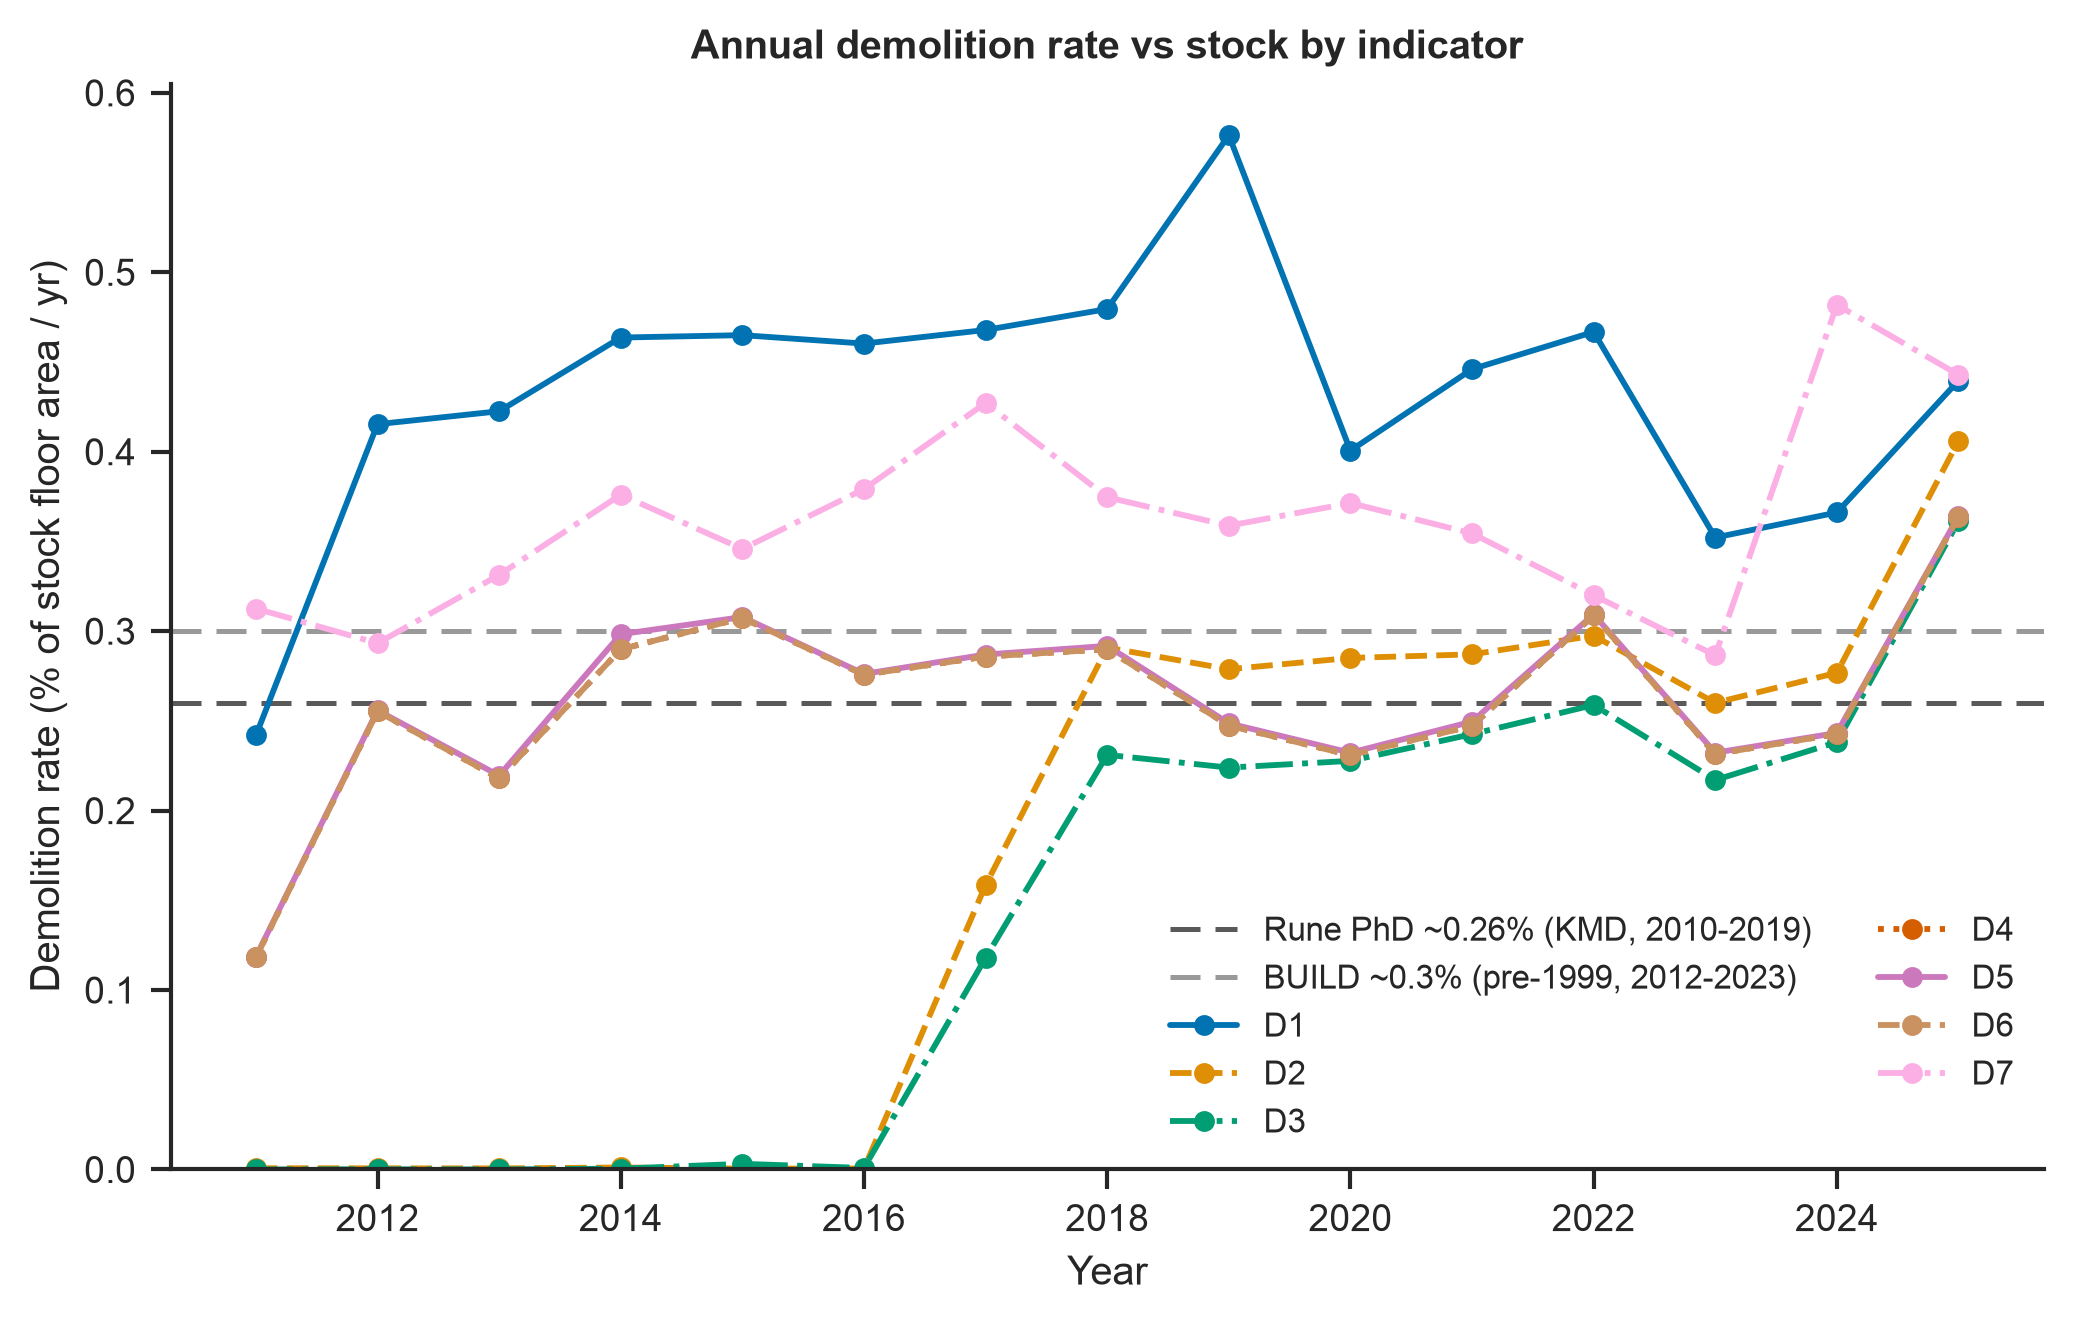
\includegraphics[width=0.7\textwidth]{media/rate_vs_stock.png}
\caption{Annual demolition rate per indicator, 2011--2025: complete-case
demolished residential-plus-commercial floor area divided by the matched
BYGB34 stock at 1~January of each year. D4 is hidden beneath D5 (their
dated annual series are identical). Dashed horizontal lines mark the
reference levels of 0.26 and 0.3\,\% per year used for the comparison
with published estimates (Section~\ref{sec:build-comparison}).}
\label{fig:rate-vs-stock}
\end{figure}

\subsection{Comparison with published rate estimates}\label{sec:build-comparison}
%% STATUS: WRITTEN 2026-07-12 from rates_summary.csv (windows 2011-2019
%%   and 2012-2023) + the published PDFs on file. Was "Comparison with
%%   BUILD"; retitled because it now also carries the KMD-based published
%%   rate. BUILD's published reference numbers (verified against the
%%   report): ~26.6 M m2 retired 2012-2023 (pre-1999 buildings) ~= 2.2 M
%%   m2/yr ~= 0.3% of 674 M m2 stock; agriculture 46% of retired area.
%% NOTE (group): the ~0.26%/yr (2010-2019) level drawn in the figure is
%%   from Rune Andersen's PhD thesis (DTU 2023), which has NO entry in
%%   references.bib — hence the \refneeded below. The citable published
%%   figure from the same extract is 0.24% (2011-2019, annual range
%%   0.20-0.28%) in \cite{andersen2022adaptation} (verified against the
%%   PDF on file, §5.1 and §6).
The published national demolition rate computed from the KMD extract of
Section~\ref{sec:kmd} is an average of 0.24\,\% of the existing
building-stock floor area per year over 2011--2019, with annual values
between 0.20 and 0.28\,\%~\cite{andersen2022adaptation}. Over the same
window, the primary pairing gives 0.254\,\% per year for D4 and D5: the
total-demolition-case family that Section~\ref{sec:kmd} shows coincides
with the extract also lands inside the published annual range. The
remaining indicators fall outside it --- D1 at 0.444\,\%, and D2 and D3 at
0.081\,\% and 0.064\,\%, the last two pulled down by their near-empty
pre-2016 series (Section~\ref{sec:rate-vs-stock}); the notification-dated
D6 \pending{recompute the D6 rate with src/rates.py after the total-only
redefinition}. A closely related KMD-based figure of
approximately 0.26\,\% per year over 2010--2019 \refneeded{Rune Andersen
PhD thesis (DTU 2023); add verified entry before citing} is drawn as a
reference level in Figure~\ref{fig:rate-vs-stock}; BYGB34 begins in
2011, so its 2010 start year cannot be matched here.

BUILD's analysis counts buildings constructed before 1999 that were
retired (``udg{\aa}et'') from the register in 2012--2023 and reports
approximately 26.6~million~m\textsuperscript{2} of retired
residential-plus-commercial floor area over those twelve years --- about
2.2~million~m\textsuperscript{2} per year, or 0.3\,\% of a
674~million~m\textsuperscript{2} stock on the same area
basis~\cite{jensen2025nedrivning}. We do not apply their construction-year
restriction, so over 2012--2023 our numerator is wider than theirs. On
that window the primary pairing runs from 0.127\,\% per year (D3) to
0.451\,\% (D1), with the total-demolition-case indicators D4/D5 at
0.266\,\% and D2 at 0.155\,\% (D6 \pending{recompute}); BUILD's
approximately 0.3\,\% lies inside this band. In absolute terms the same
window gives 0.9--3.0~million~m\textsuperscript{2} per year across the
indicators (case family 1.8), around BUILD's approximately
2.2~million~m\textsuperscript{2} per year.
\groupdecision{Methods Section~\ref{sec:comparisons} still announces a
reproduction of BUILD's exact setup (pre-1999 buildings only); the
comparison above applies no construction-year cut (decided 2026-07-12).
Align the Methods text, or decide whether the exact-setup run is still
wanted.}
